\documentclass[a4paper,11pt]{ltjsarticle}
\usepackage{amsmath,amssymb}
\usepackage{geometry}
\usepackage{enumitem}
\usepackage{graphicx}
\usepackage{booktabs}
\geometry{margin=25mm}

\title{党勢推移指数を作ってみた話(第0回)}
\author{}
\date{}

\begin{document}
\maketitle

\section*{きっかけ}

ある政党の党首が党勢の低下を「謀略だ」と主張する一方、支持者は「まだ伸びている」と言っていました。実際どちらが正しいのか、自分で客観的に確かめられる指標が欲しくなったのが出発点です。SNSの言及数は自作自演も混ざりますし、世論調査は「支持政党なし」の割合が大きすぎて実態を反映しません。最終的に政党の力は選挙で獲得した議席に収束するはずなので、実際の選挙結果だけから機械的に指標を作ることにしました。

\section*{指数の設計}

作ったのは $C_p(T)$ という指数です。式で書くとこうなります。

\[
C_p(T) = \frac{\sum_{e \in T} \sqrt{n_e P_e} \phi_p(e)}{\sum_{e \in T} \sqrt{n_e P_e}}。
\]

記号の意味は次の通りです。

\begin{itemize}[nosep]
\item $e$: 期間 $T$(直近12か月)のあいだに投票が行われた選挙(衆院・参院・都道府県議会・市区町村議会・都道府県知事・市区町村長選が対象)
\item $P_e$: その選挙$e$が代表する人口(国会なら全国人口、それ以外はその自治体の人口)
\item $n_e$: その選挙$e$で決まる議席・ポストの数(都道府県知事・市区町村長は常に1、それ以外は実際の議席数)
\item $\phi_p(e)$: その選挙 $e$ で政党 $p$ が獲得した実効的なシェア(首長選挙は推薦を含む)
\end{itemize}

1回の選挙で複数の議席が同時に決まる選挙(衆院・参院・都道府県議会・市区町村議会)だけ、議席数 $n_e$ は$1$より大きくなります。都道府県知事・市区町村長は1自治体につき1人なのに対し、これらの選挙は一度に複数(国政選挙なら数百人分)の議席が決まるからです。$n_e$ はその選挙で実際に決まった議席数そのものです(衆院選なら465議席、参院選の半数改選ならその回の改選議席数で近年は124議席、地方議会ならその自治体の定数)。衆参を合わせた値ではありません。衆院選と参院選は別々の選挙イベントとして、それぞれ自分の $n_e$ で扱います。

人口を線形にそのまま重みにすると大都市の一票が地方の何千倍にもなってしまい、かといって完全に均等重みにすると単に自治体の「数」が多い方が勝つ勝負になってしまいます。そこで「ペンローズの平方根則」を前提に重みをつけています。

平方根則を知っている前提で、なぜ$\sqrt{n_e P_e}$とするのかという理由について説明します。人口の平方根だけで重みをつける(つまり分子を$\sum_{e \in T} \sqrt{P_e} \phi_p(e)$にする)と、数百人いる当選者全体がどこかの首長1人と同格の「1票」になってしまいます。
そこで、当選者・首長を全員どこかに集めてきて多数決させる、という仮想的な状況を考えましょう。国会議員も地方議員も知事・市区町村長と同じ「1人の代表」として扱うのが自然です。ある衆院選または参院選$e$で決まる $n_e$ 人の当選者は、全員合わせて全国人口 $P_{全国}$ を代表しているので、1人あたりの代表人口は $P_{全国}/n_e$ です。首長と同じ「代表人口の平方根」を重みにすると、当選者1人の重みは $\sqrt{P_{全国}/n_e}$ になります。
このとき、政党 $p$ が獲得した議席数は $n_e\phi_p(e)$ 人です(全当選者 $n_e$ 人のうち、政党 $p$ のシェアが $\phi_p(e)$ なので)。政党 $p$ の当選者全員ぶん重みを足し合わせると、

\[
n_e\phi_p(e) \times \sqrt{\frac{P_{全国}}{n_e}}  = \phi_p(e)\sqrt{n_e P_{全国}}、
\]

となり、これが指数の分子に現れる $\sqrt{n_e P_e} \phi_p(e)$ の由来です。

集計期間を直近12か月の後方ウィンドウにしているのは、統一地方選のように選挙が特定の月に集中する季節性を、どの時点で切っても機械的にキャンセルできるからです。単月だけで集計すると、選挙が1件しか無い月とその月にたまたま無所属ばかり当選した月とで指数が極端に振れてしまいます。

都道府県議会・市区町村議会の選挙も対象に含めています。自民党系候補の多くが地方議会選挙で党名を出さず無所属で出馬する一方、共産党はほぼ必ず党名を出すという慣行があり、単純に政党間で比較すると歪みが出ることを実際のデータで確認しています。ただしこれは「A党とB党のどちらが大きいか」という比較を歪めるだけで、後述の通りこの指数はそもそも政党間の比較用ではなく各政党自身の推移を見るためのものなので、実害にはなりません。首長選挙のような推薦・支持政党による補正は地方議会の候補者個人には行っておらず、届出政党をそのまま使います(国会の選挙と同じ扱いです)。

個別に追跡する政党は、政党助成法上の「政党要件」(国会議員5人以上、または直近の国政選挙で得票率2\%以上)を満たす政党だけです。それ以外は無所属とまとめて扱います。

\section*{現在の指数の値(2026年9月時点)}

$C_p(T)$は前月以前のデータと比較してこそ意味を持つ指標です。実際にパイプラインを動かし始めた2026年9月より前の期間についても、月次で過去に遡って再構成できます。パイプラインが遡れる限界(地方自治総合研究所の推薦・支持データが2018年版までしかない)まで遡ると、2018年1月〜2026年9月の全期間(105か月、いずれも12か月後方ウィンドウ)を再構成できます。

ただし、政党どうしを比べるのには注意が必要です。上で触れた「自民党系候補は地方選挙で党名を出さず無所属で出馬しやすく、共産党はほぼ必ず党名を明示する」という慣行の非対称性は、地方議会を対象から外しても完全には消えません。首長選でも同じ傾向があり、推薦・支持政党のデータである程度は補正していますが、直近の公開遅れ(後述)もあって補正しきれない分が残ります。そのため、\textbf{ある時点でA党とB党のどちらが大きいか}という比較は割り引いて読む必要があります。一方、\textbf{同じ政党の値が時間とともにどう動いたか}は、その政党自身の「党名を隠す度合い」が大きく変わっていない限り意味を持ちます。

そこで以下は、政党ごとに高さを正規化した党勢推移指数の推移(上段)、同じ時間軸における選挙の種類ごとの重みシェアの推移(中段)、そして首相の在任期間(下段)を並べたグラフです。上段は政党間の高さ(絶対的な水準)を比べる意図はありませんが、複数の政党が同じ時期にどう動いたか(タイミングの一致)は、実際に同じ選挙が複数の政党を同時に動かしている以上、素直に読み取れます。中段は、その「同じ時期」を引き起こしている選挙の種類を、重み$\sqrt{n_eP_e}$の合計に占める割合として選挙の種類(衆院選・参院選・都道府県知事・都道府県議会・市区町村長・市区町村議会)ごとに分解したものです。

\begin{center}
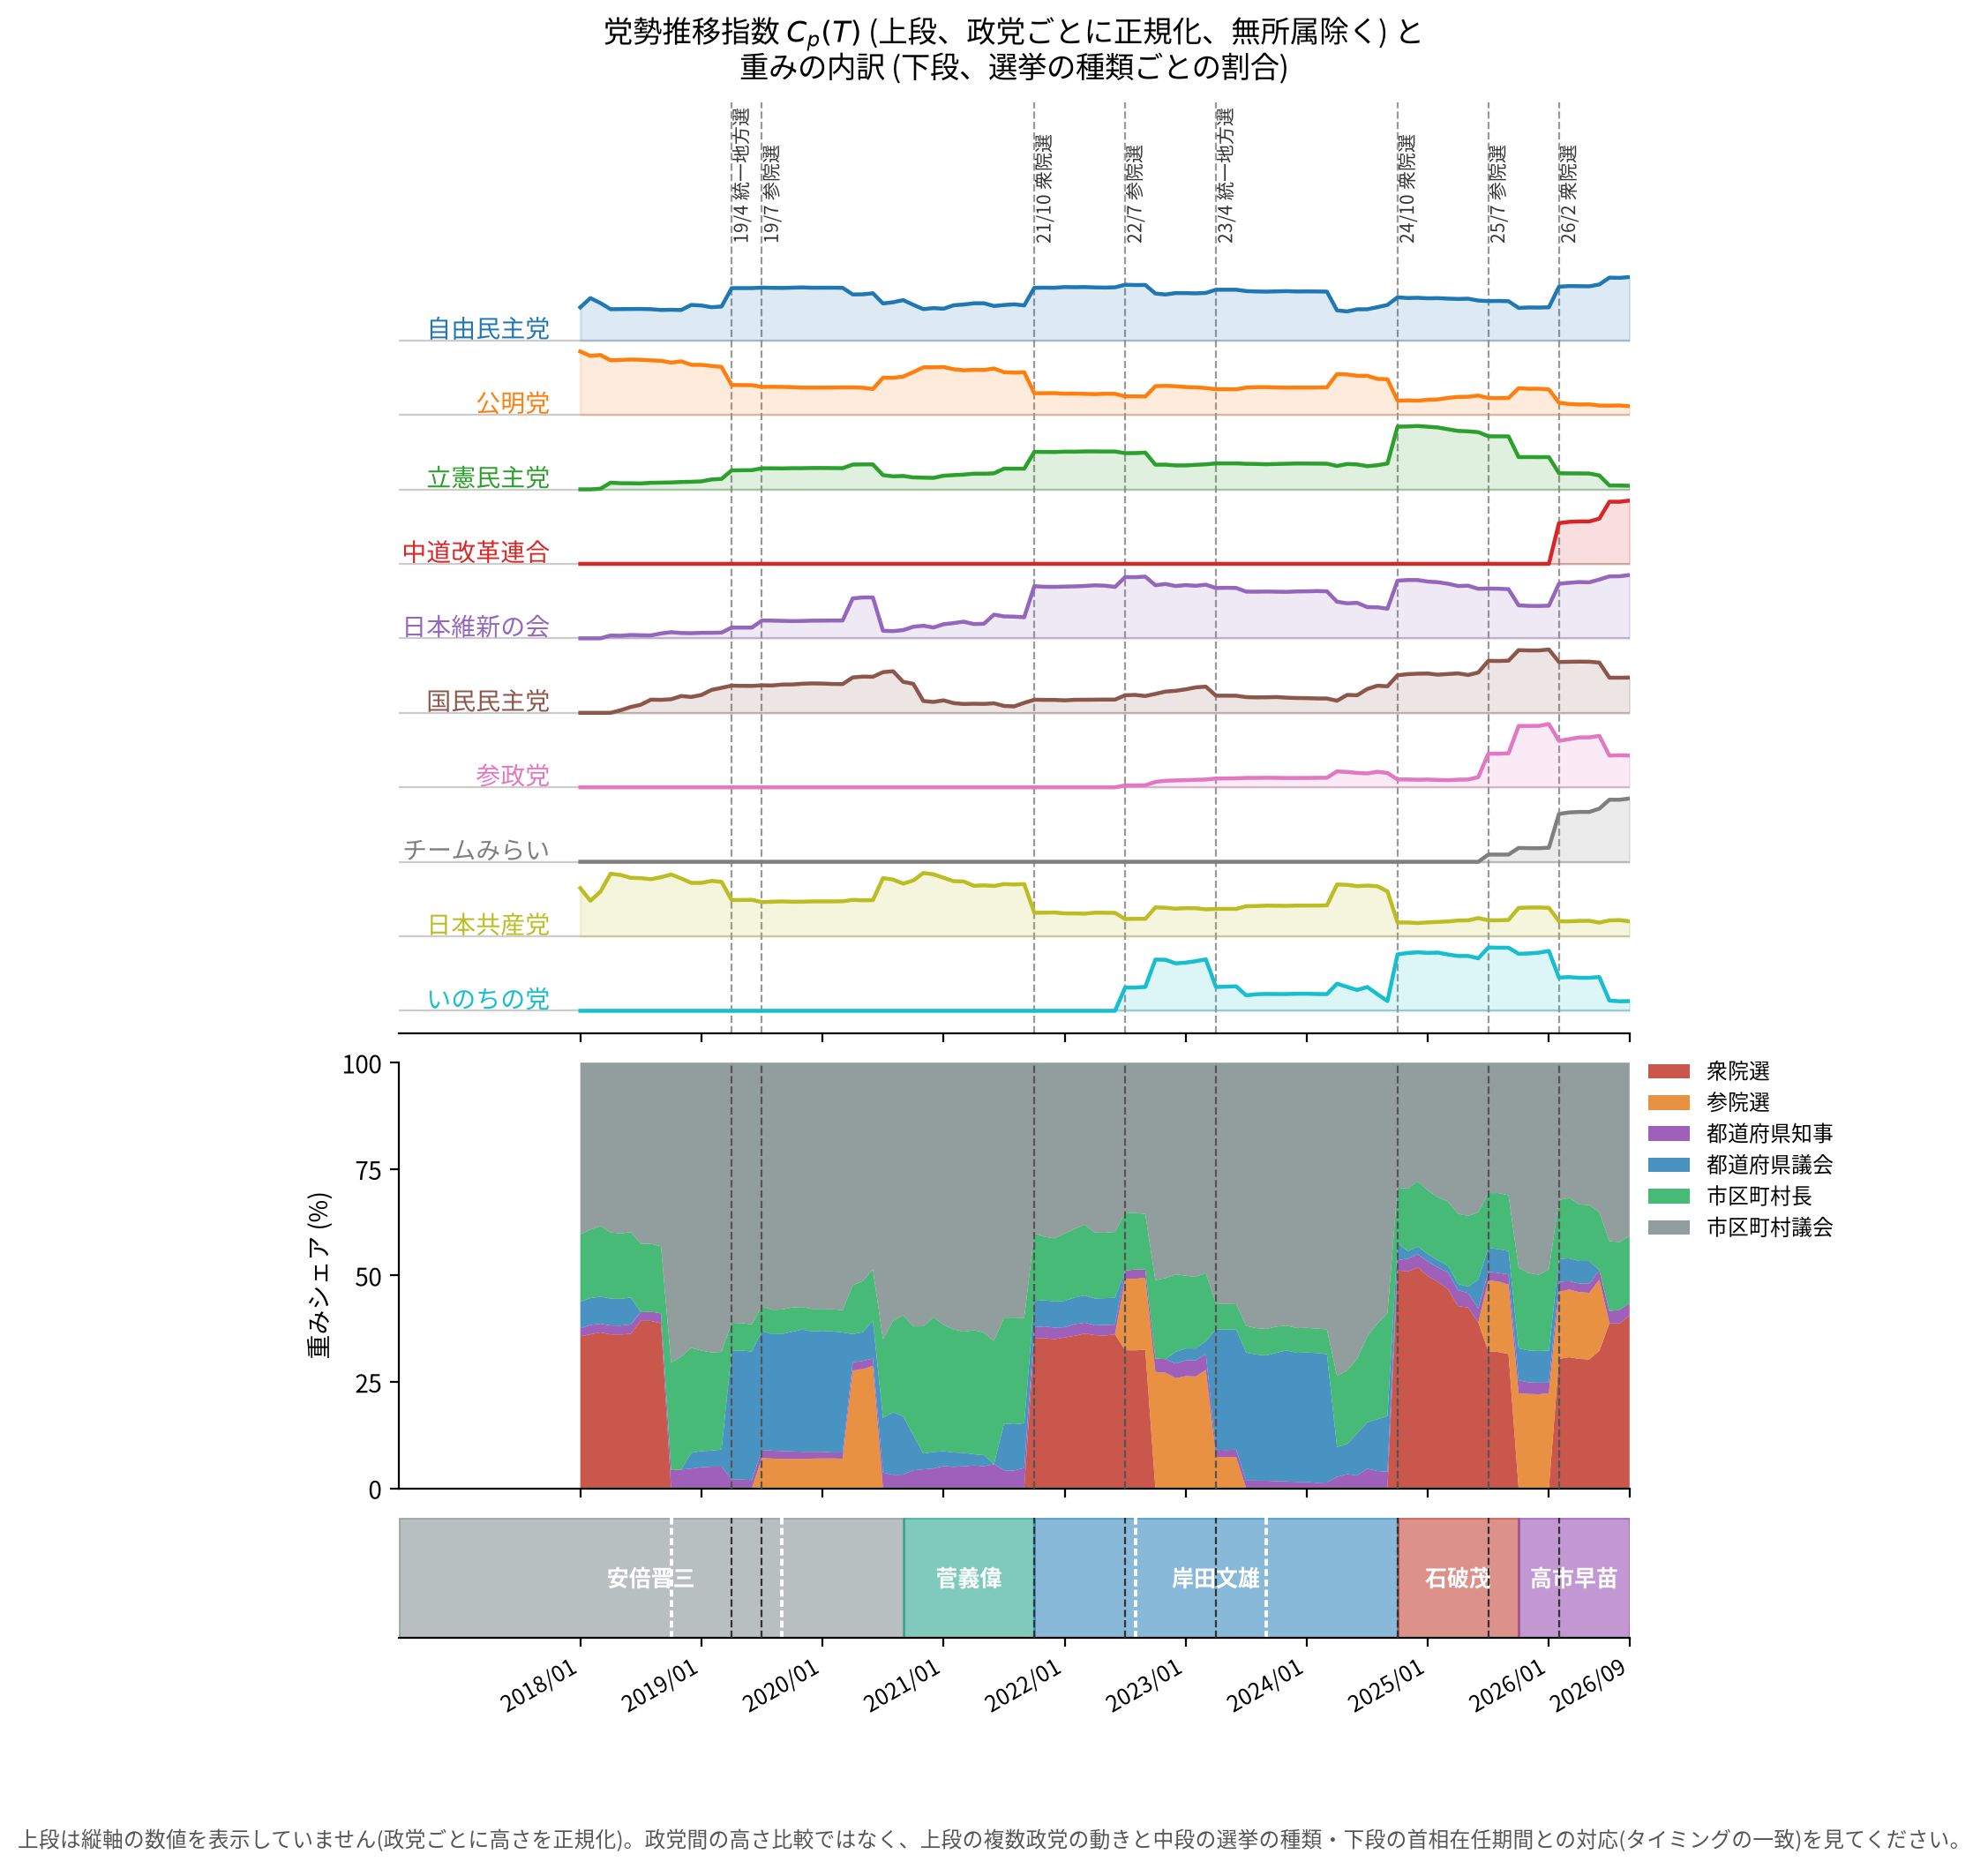
\includegraphics[width=0.95\textwidth]{images/cp_and_level_share.png}
\end{center}

無所属は直近数か月ぶんのデータ公開に構造的な遅れがあり、素の値では過大に出ます。加えて地方議会(特に市区町村議会)は無所属で出馬する候補がもともと多く、2026年9月時点で無所属の素の値は48.0\%に達します。上段のグラフは無所属を除いて正規化した値です。

上段のグラフ全体を貫くのこぎり状の動きは、国政選挙(または都道府県議会選挙のように一斉改選される選挙)が12か月ウィンドウに入るたびに指数がその選挙結果へ大きく振れ、ちょうど12か月後にその選挙がウィンドウから抜けると反動で戻る、という機械的な挙動です。都道府県議会は統一地方選のたびに一斉改選されるため、国政選挙と同じこの挙動を示します。個別の山谷は、それぞれの政党自身の推移として実際の選挙で説明できます。

中段を見ると、市区町村議会は全期間を通じて27.9\%を下回ったことがなく、指数の基盤として常に一定の割合を保ち続けています。一方、衆院選(0\%〜51.9\%)・参院選(0\%〜28.8\%)・都道府県議会(0\%〜30.8\%)は、一斉改選が行われた月の前後だけ急激に割合が高まり、それ以外の月ではゼロに近づきます。都道府県知事(1.3\%〜5.7\%)と市区町村長(5.2\%〜31.7\%)は、任期が自治体ごとにばらけているため、この中間的な挙動を示します。

このように、特定の選挙の種類が指数を単独で支配し続ける期間は存在しません。都道府県議会選挙を新たに指数へ組み込んだことで変動幅そのものは大きくなりましたが、それは衆院選・参院選がもともと示していた挙動と同種のものであり、指数の妥当性を損なうものではないと判断しています。

下段は首相の在任期間で、白の点線は政権交代を伴わない内閣改造(2018年10月・2019年9月の安倍改造内閣、2022年8月・2023年9月の岸田改造内閣)の時期を示しています。首相交代そのもの(2020年9月・菅義偉、2021年10月・岸田文雄、2024年10月・石破茂、2025年10月・高市早苗)は、いずれも衆院選と同時期か、その選挙結果を受けた特別国会での指名によるものです。実際、2021年10月・2024年10月・2026年2月の首相交代は上段・中段の急変時期とそのまま重なる一方、政権交代を伴わない内閣改造の時期には、指数に対応する目立った変動は見られません。首相個人の交代ではなく、あくまで選挙結果が指数を動かしていることの傍証です。

\begin{itemize}
\item \textbf{2019年4月・統一地方選}: 公明党が約39\%→24\%に急落、自民党が約31\%→48\%に急伸。
\item \textbf{2021年10月・衆院選(岸田政権発足後初の総選挙)}: 自民党が約32\%→48\%に急伸、公明党は約35\%→18\%に急落。
\item \textbf{2024年4月・地方選挙}: 公明党が約22\%→33\%に急伸(国政選挙の無い月だが、その月の地方選挙51件の中で公明党が18.2\%という異例の強さを見せた。地方選挙単独でも指数が動く一例)。
\item \textbf{2024年10月・衆院選(石破政権発足後の総選挙)}: 自民党が約32\%→39\%に急伸する一方、公明党は約29\%→12\%に急落(同月は公明党代表の落選を含む苦戦が実際に報じられており、指数の急落と整合する)。ただしこの急伸は自民党自身の躍進ではありません。実際の議席は259から191へ減り、公明党との連立過半数も失っています。野党側の議席が立憲民主党148・日本維新の会38・国民民主党28などに分散したうえ、れいわ新選組・社民党・日本保守党(あわせて12議席)は直近では政党要件を満たさず追跡対象から外れているため、追跡対象政党どうしの相対シェアでは自民党が単独最大のまま押し上げられた、という指数特有の見え方です。
\item \textbf{2026年2月・衆院選+中道改革連合の結成}: 立憲民主党・公明党が統一名簿で合流して中道改革連合を結成し、自民党が約30\%→49\%に急伸。
\end{itemize}

\subsection*{カバレッジ(データの網羅率)}

上記の指数は、既知の首長のうち都道府県知事47/47(100\%)・市区町村長1738/1788(97.2\%)をカバーした時点の値です。総務省の年次集計だけでは個々の自治体を特定できないため、選挙ドットコム・Wikidataを組み合わせて自治体ごとに直接クロールしています。残り4自治体はクロール自体が構造的に失敗するため、97.2\%が実質的な上限です。

この97.2\%を基準値とし、目立って下回った場合はクロール処理に不具合が起きている可能性が高いとみなしてコードを見直します。実行のたびに自動記録する仕組みは用意済みですが、グラフ化するにはまだ月数が足りないため、数字が動いた時にあらためて紹介します。

\subsection*{予測とサプライズについて}

第0回のうちに、今後の月次記事で「予測」欄を書くための裏付けを示しておきます。実際に機械学習モデルで$C_p(T)$の来月の値を予測できるかを検証し、その結果に基づいて予測方針を決めました。

使ったのはTimesFM-3です。Google Researchが2026年8月に公開した時系列予測の基盤モデルで、追加学習なしにゼロショットで予測でき、国政選挙のような既知の将来イベントを条件(covariate)として与えられるのが特徴です。

比較したのは3通りの予測です。「前月から変化なし」とするゼロ予測、「前月の差分をそのまま今月も継続する」とするモメンタム予測、そしてTimesFM-3です。国政選挙が絡まない平常月では、ゼロ予測が最も当たり、モメンタム予測・TimesFM-3を使うとむしろ悪化しました。国政選挙が絡む月(実際に選挙があった月と、その12か月後にウィンドウから抜ける月、あわせて9か月分)に限って集計した結果は次の通りです(値は月次差分の平均絶対誤差を100倍したもの、小さいほど当たっている)。

バックテストの対象は、期間全体を通じて安定した時系列を持つ6党(自由民主党・公明党・立憲民主党・日本維新の会・国民民主党・日本共産党)に絞っています。TimesFM-3が予測の文脈として使う36か月分の履歴が必要なため、これに満たない政党は検証できません。参政党は政党要件を満たした2024年10月から24か月分、中道改革連合・チームみらいは結成された2026年2月からいずれも8か月分しか履歴が無く、この条件を満たしません。いのちの党は履歴自体は長いものの、政党要件を満たしたり失ったりを繰り返しており(直近では2020年8月〜2022年7月の24か月間、要件を満たさず追跡対象から外れています)、安定した時系列として扱えません。

\begin{center}
\begin{tabular}{lccc}
\toprule
政党 & ゼロ予測 & モメンタム & TimesFM-3 \\
\midrule
自由民主党 & 3.89 & 3.81 & 4.39(悪化) \\
公明党 & 9.25 & 9.70 & \textbf{5.28(43\%改善)} \\
立憲民主党 & 3.83 & 3.73 & 3.77(ほぼ同等) \\
日本維新の会 & 3.79 & 3.78 & \textbf{3.33(12\%改善)} \\
国民民主党 & 0.99 & 1.70 & 1.07(悪化) \\
日本共産党 & 0.57 & 1.20 & 0.51(ほぼ同等) \\
\bottomrule
\end{tabular}
\end{center}

公明党・日本維新の会の2党だけTimesFM-3がゼロ予測を明確に上回り、自由民主党・国民民主党はむしろ悪化しました。そこで今後の月次記事では、国政選挙月の公明党・日本維新の会だけモデルの予測値を使い、それ以外(バックテスト対象外の参政党・中道改革連合・チームみらい・いのちの党を含む)は「変化なし」を予測値とします。参政党などが36か月分の履歴を蓄積した時点で、追加の検証対象に加える予定です。実際の値との差分(サプライズ)は毎月確認しますが、差分が大きいこと自体は「国政選挙側の想定超過」「地方選挙単独の動き」のいずれもありえるため(上記の2024年4月の例が典型)、単月の生データまで遡って裏取りする一手間を挟みます。

\textbf{来月(2026年10月)の予測}: 2026年10月に予定されている国政選挙は無いため、上記の採用ルールに従いゼロ予測(差分0、つまり2026年9月とほぼ同じ水準が続く)を採用します。実際の結果は第1回で答え合わせします。

\section*{データソース}

衆参の議席・地方議会の議席・首長の選挙結果・推薦支持政党データは、それぞれ次のソースから取得しています。

\begin{itemize}[nosep]
\item 衆参の議席: 各院の公式サイト
\item 都道府県議会・市区町村議会の議席: 選挙ドットコム(自治体ごとの個別選挙結果)
\item 都道府県知事・市区町村長の選挙結果: 総務省の統計をベースに、選挙ドットコム・Wikidataを組み合わせて選挙のたびに反映(総務省の集計だけでは更新が年1回に留まるため)
\item 無所属で当選した首長の実質的な支持政党: 地方自治総合研究所が公開している推薦・支持政党データ
\end{itemize}

上記のグラフに添えた首相の在任期間・内閣改造の時期は指数の算出には使っておらず、文脈として示す参考情報です。首相官邸の公式発表・報道をもとにしています。

どのデータをどう使っているかは設計文書としてまとめてあり、算出コードとあわせて誰でも検証できる形で公開する予定です。

\section*{著作権について}

算出コードはMITライセンスで公開し、自由に使ってもらって構いません。ただしこの記事や設計文書など、文章そのものの著作権は放棄していません。

\section*{AI活用について}

指数の設計・データソース調査・実装には、AI(Claude)を活用しています。透明性を大事にしたいプロジェクトなので、そのこと自体もここに明記しておきます。

\section*{今後について}

更新は月1回を目安にします。あくまで個人の趣味の定点観測です。コメント欄は閉じています。次回以降は次の4本立てで淡々と続けていく予定です。

\begin{enumerate}[nosep]
\item 直近月の選挙概況
\item 前回書いた翌月予測の答え合わせ
\item 大きな動きがあれば予測と比較して実際にサプライズだったのか裏取り
\item 次の月の予測
\end{enumerate}

\end{document}
